\documentclass{article}
\usepackage[a4paper]{geometry}
\usepackage[english]{babel}
\usepackage[utf8]{inputenc}
\usepackage{url}
\usepackage{hyperref}
\usepackage{graphicx}
\usepackage{amssymb}
\usepackage{amsmath}
\usepackage{amsfonts}
\usepackage{xspace}
\usepackage{yfonts}
\usepackage{mathrsfs}

\title{Computational Project - Theme Proposal}
\author{
	Luiz Fernando Bueno Rosa - RA: 221197 \\
	Lucas Guesser Targino da Silva - RA: 203534
}

\newcommand{\nphard}{NP-hard\xspace}

\newcommand{\real}{\ensuremath{\mathbb{R}}\xspace}
\newcommand{\realnonnegative}{\ensuremath{\mathbb{R}_{+}}\xspace}
\newcommand{\realpositive}{\ensuremath{\mathbb{R}_{+}^{*}}\xspace}
\newcommand{\nrealnonnegative}[1]{\ensuremath{\mathbb{R}_{+}^{#1}}\xspace}
\newcommand{\nrealpositive}[1]{\ensuremath{\mathbb{R}_{+}^{*#1}}\xspace}

\newcommand{\true}{\ensuremath{true}\xspace}
\newcommand{\false}{\ensuremath{false}\xspace}

\newcommand{\abs}[1]{\ensuremath{\left| #1 \right|}\xspace}
\newcommand{\tuple}[1]{#1-tuple\xspace}
\newcommand{\Set}[1]{\ensuremath{\left\{#1\right\}}}
\newcommand{\SetOf}[2]{\ensuremath{\left\{ #1 : #2 \right\}}\xspace}
\newcommand{\OrderedSet}[1]{\ensuremath{\langle#1\rangle}\xspace}
\newcommand{\function}[3]{\ensuremath{#1: #2 \rightarrow #3}\xspace}

\newcommand{\bigo}[1]{\ensuremath{\mathcal{O}\left( #1 \right)}}

\newcommand{\vehicleO}{\ensuremath{\upsilon}\xspace}
\newcommand{\vehicleSet}{\mathcal{V}\xspace}
\newcommand{\loadingFunction}{\ensuremath{\eta}\xspace}
\newcommand{\loadingFunctionApply}[1]{\loadingFunction \left( #1 \right)\xspace}
\newcommand{\loadingLimit}{\ensuremath{L}\xspace}
\newcommand{\nAxles}{\ensuremath{\alpha}\xspace}
\newcommand{\loadingCodomain}{\nrealnonnegative{\nAxles}}

\newcommand{\itemO}{\ensuremath{\iota}\xspace}
\newcommand{\itemSet}{\ensuremath{\mathcal{I}}\xspace}
\newcommand{\itemDomain}{\ensuremath{\nrealpositive{3} \times \nrealnonnegative{3}}\xspace}

\newcommand{\containero}{\ensuremath{c}\xspace}
\newcommand{\containerSet}{\ensuremath{\mathcal{C}}\xspace}

\newcommand{\lx}{\ensuremath{\chi}\xspace}
\newcommand{\ly}{\ensuremath{\psi}\xspace}
\newcommand{\lz}{\ensuremath{\omega}\xspace}
\newcommand{\px}{\ensuremath{x}\xspace}
\newcommand{\py}{\ensuremath{y}\xspace}
\newcommand{\pz}{\ensuremath{z}\xspace}

\newcommand{\itemInput}{\ensuremath{\mathit{I}_{o}}\xspace}
\newcommand{\itemOutput}{\ensuremath{\mathit{I}_{f}}\xspace}
\newcommand{\stackingPredicateSymbol}{\ensuremath{\mathcal{SC}}\xspace}
\newcommand{\stackingPredicate}[1]{\ensuremath{\stackingPredicateSymbol \left( #1 \right)}\xspace}

\newcommand{\vehicleInput}{\vehicleO}

\newcommand{\constraintsPredicateSymbol}{\ensuremath{\mathscr{C}}\xspace}
\newcommand{\constraintsPredicate}[1]{\ensuremath{\constraintsPredicateSymbol \left( #1 \right)}\xspace}

\begin{document}

\maketitle

\section{Motivation}

Consider the problem of allocating items into the containers of a vehicle. In most practical cases, in order for those allocations to be of any practical use, they must take into account the loading on the axle of the vehicle. That is important for several reasons:

\begin{enumerate}
	\item countries have regulations on how much weight each type of axle can have \cite{bib:law-loading-on-axles};
	\item excess of loading on the axles of a vehicle can decrease its lifespan or cause a direct damage to the vehicle;
	\item heavy unbalanced cargos unstabilize the vehicle that carries it, increasing the risk of accidents;
\end{enumerate} 

Those problems in the packing family are know to be \nphard \cite{bib:knapsack-problems}. For such reason, in practice, one is usually more interested in finding an acceptable solution in a reasonable amount of time rather than the optimal one. In such situations, heuristics become a required technique.

When designing heuristics, it is usually difficult to optimize for several objectives at the same time, usually because they conflict with each other. One possible approach for such problems is to design a heuristics for one of them and make a post-processing on the found solution in order to find a compromise between the others. Such approach is very attractive in practice because it allows one to both reuse and extend solutions for similar problems, cutting development and testing costs.

The problem we propose here is a post-processing algorithm used in the context above: one has a solution for the knapsack problem but it must be adapted to satisfy an extra constraint. In the case we propose here, it is given to us an allocation of items in a vehicle and we must remove the items so to satisfy limits of loading on the axles minimizing the number of items to be removed.

In the next sections, we provide a detailed formulation of such problem.

\begin{figure}
	\centering
	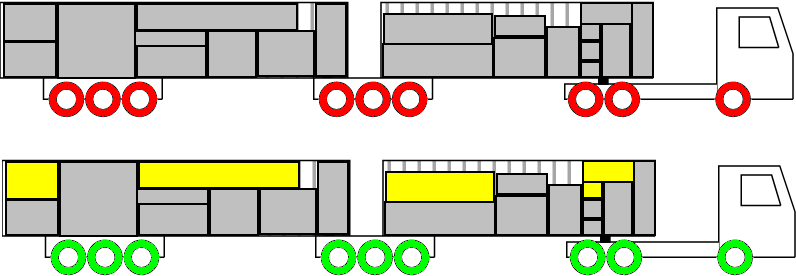
\includegraphics[width=\textwidth]{images/example_remove_items_from_vehicle.png}
	\caption{Above an item with a cargo which exceeds the loading on its axles. Below, when the yellow items are removed, the loading on the axles constraint is satisfied.}
	\label{fig:example remove items}
\end{figure}

\section{Definitions}

\subsection{Item}

An \textbf{Item} \itemO is a \tuple{6}:

\begin{equation}
	\label{definition:item}
	\itemO = \OrderedSet{
		\lx,
		\ly,
		\lz,
		\px,
		\py,
		\pz
	}
\end{equation}

in which the components represent the item's\footnote{See a definition for ``dimension'' in \cite{bib:dict-dimension}}:

\begin{enumerate}
	\item $\lx \in \realpositive$: dimension in the \px direction;
	\item $\ly \in \realpositive$: dimension in the \py direction;
	\item $\lz\in \realpositive$: dimension in the \pz direction;
	\item $\px \in \realnonnegative$: x position;
	\item $\py \in \realnonnegative$: y position;
	\item $\pz \in \realnonnegative$: z position;
\end{enumerate}

We represent by $\itemSet = \itemDomain$ the set of all items.

The reason an items is seen in that way is because of the stacking

%\subsection{Container}
%
%A \textbf{Container} \containero is a \tuple{3}:
%
%\begin{equation}
%	\label{definition:container}
%	\containero = \OrderedSet{
%		\lx,
%		\ly,
%		\lz
%	}
%\end{equation}
%
%in which the components represent the container's:
%
%\begin{enumerate}
%	\item $\lx \in \realpositive$: dimension in the \px direction (the length);
%	\item $\ly \in \realpositive$: dimension in the \py direction (the width);
%	\item $\lz \in \realpositive$: dimension in the \pz direction (the height);
%\end{enumerate}

\subsection{Vehicle}

A Vehicle \vehicleO is a \tuple{3}:

\begin{equation}
	\label{definition:vehicle}
	\vehicleO = \OrderedSet{
		\nAxles,
		\loadingFunction,
		\loadingLimit
	}
\end{equation}

in which:

\begin{enumerate}
	\item $\nAxles$ is the number of components of the vehicle's loadings;
	\item $\function{\loadingFunction}{\itemSet}{\loadingCodomain}$: a function that associates every item to a vehicle's loading;
	\item $\loadingLimit \in \loadingCodomain$: represents the vehicle's loading limit;
\end{enumerate}

We represent by $\vehicleSet$ the set of all vehicles.

\section{Problem Statement}

\subsection{Input}

\begin{enumerate}
	\item $\itemInput \subseteq \itemSet$: the set of items
	\item $\vehicleInput \in \vehicleSet$: the vehicle
\end{enumerate}

\subsection{Constraints}

\subsubsection*{Loading Limit Constraint}
\begin{equation}
	\label{constraint:loading-limit}
	\displaystyle\sum\limits_{\itemO \in \itemInput}
		\loadingFunctionApply{\itemO}
		\leq \loadingLimit
\end{equation}

\subsubsection*{Stacking Constraint}
\begin{equation}
	\label{constraint:stacking}
	\mbox{An item can only be removed if all items above it have already been removed}
\end{equation}

We represent whether such constraint is satisfied or not by $\stackingPredicate{\itemOutput} \in \Set{\true, \false}$

\subsection{Output}

A subset $\itemOutput \subseteq \itemInput$ of the input items.

\subsection{Objective}

\begin{equation}
	min\SetOf{\abs{\itemInput} - \abs{\itemOutput}}{\itemOutput \subseteq \itemInput \ \land \ \constraintsPredicate{\itemOutput}}
\end{equation}

Minimize the number of items removed so that all constraints are satisfied.

% ----------- REFERENCES -----------
\bibliographystyle{unsrt}
\bibliography{bibliography}

\end{document}
